\documentclass[12pt,letterpaper]{hmcpset}
\usepackage[margin=1in]{geometry}
\usepackage{graphicx}
\usepackage{zach}
\usepackage{enumitem}
\usepackage{tikz}

\usetikzlibrary{%
  arrows,%
  calc, %
  fit, %
  shapes.misc,% wg. rounded rectangle
  shapes.arrows,%
  chains,%
  matrix,%
  positioning,% wg. " of "
  scopes,%
  decorations.pathmorphing,% /pgf/decoration/random steps | erste Graphik
  shadows%
}

% info for header block in upper right hand corner
\name{Zachary Seymour}
\class{CS 520--03}
\assignment{Homework 1}
\duedate{September 30, 2013}

\begin{document}

\problemlist{}

\begin{problem}[1]
Before we start this code sequence, assume that the registers R1 through R6 contain, respectively, the values of 100, 200, 300, 400, 500 and 600.  Assume further that the instructions are 4 Bytes wide, the memory is byte-addressable (that is, each byte in the memory has a unique address) and the address of the first \texttt{LOAD} instruction is 5000.  This means that the \texttt{ADD} instruction is stored at address 5004, the SUB at address 5008 and so on.  The \texttt{LOAD} and \texttt{STORE} write and retrieve one 4-Byte wide memory word, whose effective address is computed by the \texttt{LOAD} and \texttt{STORE}.  Assume that the contents of the memory words targeted by the first and second \texttt{LOAD} instructions are 3205 and 6409, respectively.

Assume that this code fragment is executed on a five-stage in-order pipeline with data forwarding, as we discussed in class. Determine how many cycles would it take to execute this code and for each cycle, show the following: contents of the register file, data at the ALU inputs, data at the ALU output.

\end{problem}

\begin{solution}
This code, considering the delay for the \texttt{LOAD} instruction, would require 10 cycles to execute.
\begin{enumerate}[label=Cycle \arabic*]
\item 

\begin{tabular}{|l|l|}
\hline
R1 & 100 \\
\hline 
R2 & 200 \\
\hline
R3 & 300 \\
\hline
R4 & 400 \\
\hline
R5 & 500 \\
\hline
R6 & 600 \\
\hline
\end{tabular}

\begin{itemize}
\item ALU inputs at Cycle 1: Unknown
\item ALU output at Cycle 1: Unknown
\end{itemize}

\item 

\begin{tabular}{|l|l|}
\hline
R1 & 100 \\
\hline 
R2 & 200 \\
\hline
R3 & 300 \\
\hline
R4 & 400 \\
\hline
R5 & 500 \\
\hline
R6 & 600 \\
\hline
\end{tabular}

\begin{itemize}
\item ALU inputs at Cycle 2: Unknown
\item ALU output at Cycle 2: Unknown
\end{itemize}

\item 

\begin{tabular}{|l|l|}
\hline
R1 & 100 \\
\hline 
R2 & 200 \\
\hline
R3 & 300 \\
\hline
R4 & 400 \\
\hline
R5 & 500 \\
\hline
R6 & 600 \\
\hline
\end{tabular}

\begin{itemize}
\item ALU inputs at Cycle 3: Unknown
\item ALU output at Cycle 3: Unknown
\end{itemize}

\item 

\begin{tabular}{|l|l|}
\hline
R1 & 100 \\
\hline 
R2 & 200 \\
\hline
R3 & 300 \\
\hline
R4 & 400 \\
\hline
R5 & 500 \\
\hline
R6 & 600 \\
\hline
\end{tabular}

\begin{itemize}
\item ALU inputs at Cycle 4: Unknown
\item ALU output at Cycle 4: Unknown
\end{itemize}

\item

\begin{tabular}{|l|l|}
\hline
R1 & 100 \\
\hline 
R2 & 200 \\
\hline
R3 & 300 \\
\hline
R4 & 400 \\
\hline
R5 & 500 \\
\hline
R6 & 600 \\
\hline
\end{tabular}

\begin{itemize}
\item ALU inputs at Cycle 5: R5 = 100 and R1=3205
\item ALU output at Cycle 5: Unknown
\end{itemize}

\item

\begin{tabular}{|l|l|}
\hline
R1 & 3205 \\
\hline 
R2 & 200 \\
\hline
R3 & 300 \\
\hline
R4 & 400 \\
\hline
R5 & 500 \\
\hline
R6 & 600 \\
\hline
\end{tabular}

\begin{itemize}
\item ALU inputs at Cycle 6: R4 = 3305 and R6=600
\item ALU output at Cycle 6: 3305
\end{itemize}

\item

\begin{tabular}{|l|l|}
\hline
R1 & 3205 \\
\hline 
R2 & 200 \\
\hline
R3 & 300 \\
\hline
R4 & 400 \\
\hline
R5 & 500 \\
\hline
R6 & 600 \\
\hline
\end{tabular}

\begin{itemize}
\item ALU inputs at Cycle 7: None
\item ALU output at Cycle 7: $3305-600=2705$
\end{itemize}

\item

\begin{tabular}{|l|l|}
\hline
R1 & 3205 \\
\hline 
R2 & 200 \\
\hline
R3 & 300 \\
\hline
R4 & 3305 \\
\hline
R5 & 500 \\
\hline
R6 & 600 \\
\hline
\end{tabular}

\begin{itemize}
\item ALU inputs at Cycle 8: None
\item ALU output at Cycle 8: None
\end{itemize}

\item

\begin{tabular}{|l|l|}
\hline
R1 & 3205 \\
\hline 
R2 & 200 \\
\hline
R3 & 300 \\
\hline
R4 & 2705 \\
\hline
R5 & 500 \\
\hline
R6 & 600 \\
\hline
\end{tabular}

\begin{itemize}
\item ALU inputs at Cycle 9: None
\item ALU output at Cycle 9: None
\end{itemize}

\item

\begin{tabular}{|l|l|}
\hline
R1 & 3205 \\
\hline 
R2 & 200 \\
\hline
R3 & 300 \\
\hline
R4 & 2705 \\
\hline
R5 & 500 \\
\hline
R6 & 600 \\
\hline
\end{tabular}

\begin{itemize}
\item ALU inputs at Cycle 10: None
\item ALU output at Cycle 10: None
\end{itemize}

\item

\begin{tabular}{|l|l|}
\hline
R1 & 3205 \\
\hline 
R2 & 200 \\
\hline
R3 & 300 \\
\hline
R4 & 6409 \\
\hline
R5 & 500 \\
\hline
R6 & 600 \\
\hline
\end{tabular}

\begin{itemize}
\item ALU inputs at Cycle 11: None
\item ALU output at Cycle 11: None
\end{itemize}



\end{enumerate}
\end{solution}

\begin{problem}[2]
Consider the execution of the following code fragment on a 5-stage in-order pipelined processor augmented with data forwarding logic.  To avoid pipeline resource conflicts, assume that every instruction goes through every pipeline stage even if some stages may not be required for them. For example, the arithmetic instructions still go through the memory stage, where their generated results are simply moved from the output latch of the ALU stage to the output latch of the memory stage. Also assume that the execution stage for each instruction takes a single cycle.
\end{problem}

\begin{problem}[2a]
Identify all of the data dependencies in this code.
\end{problem}

\begin{solution}
The second argument of the first \texttt{ADD} instruction is dependent on the result from the \texttt{SUB}.
The location accessed for the \texttt{STORE} is dependent on that produced by the first \texttt{ADD}, and the value loaded into R3 is dependent on the \texttt{STORE} before it.
Finally, the last \texttt{ADD} must wait for the load to complete for its first operand.
\end{solution}

\begin{problem}[2b]
Which of these dependencies would impact the correctness of this program if data forwarding was not implemented and no other mechanism to handle data dependencies was in place?
\end{problem}

\begin{solution}
The dependency on \texttt{SUB} from the first \texttt{ADD} would impact the correctness, because \texttt{ADD} would be fetching the value from R4 before \texttt{SUB} had written the new correct value.
Also, without hazard detection or the like, the second \texttt{ADD} would not have the correct first parameter without waiting on \texttt{LOAD} to complete execution.
\end{solution}

\begin{problem}[2c]
How many cycles does it take to execute the above code? Explain your answer.
\end{problem}

\begin{solution}
The above code requires 10 cycles to complete.  In particular, with data forwarding, the first four instructions complete in normal pipelined fashion.  With hazard detection, a bubble must be introduced on the final \texttt{ADD} instruction to wait for \texttt{LOAD} to complete, so it must wait one additional instruction longer until the value is written to the register file, resulting in 10 total cycles.
\end{solution}

\begin{problem}[2d]
For \emph{each processing cycle}, show which registers are read and written.
\end{problem}

\begin{solution}
\begin{enumerate}[label=Cycle \arabic*]
\item
\begin{itemize}
\item Read: None
\item Written: None
\end{itemize}

\item
\begin{itemize}
\item Read: R2 and R5
\item Written: None
\end{itemize}

\item
\begin{itemize}
\item Read: R2 and R4
\item Written: None
\end{itemize}

\item 
\begin{itemize}
\item Read: R4
\item Written: None
\end{itemize}

\item
\begin{itemize}
\item Read: R4
\item Written: R4
\end{itemize}

\item
\begin{itemize}
\item Read: R3 and R5
\item Written: R4
\end{itemize}

\item
\begin{itemize}
\item Read: R3 and R5
\item Written: None
\end{itemize}

\item
\begin{itemize}
\item Read: None
\item Written: R3
\end{itemize}

\item
\begin{itemize}
\item Read: None
\item Written: None
\end{itemize}

\item
\begin{itemize}
\item Read: None
\item Written: R5
\end{itemize}

\end{enumerate}
\end{solution}

\begin{problem}[2e]
For \emph{each processing cycle}, list all pairs of registers that are being compared by the forwarding logic. Show how many of these comparisons result in a match. Also indicate if any of the matches are ignored for the purpose of controlling the MUXes in front of the ALU and explain why.  
\end{problem}

\begin{solution}
\begin{enumerate}[label=Cycle \arabic*]
\item
Registers: None

\item
Registers: none

\item
Registers:
\begin{enumerate}
\item R4
\item R4
\item R4
\item R6
\end{enumerate}
Both the first-third and second-third pairs match.

\item
Registers:
\begin{enumerate}
\item ---
\item R4
\item R4
\item R3
\end{enumerate}
The second and third match.

\item
Registers:
\begin{enumerate}
\item ---
\item ---
\item R3
\item R4
\end{enumerate}
No matches.

\item
Registers: None

\item
Registers: None

\item
Registers: None (no future commands to check)

\item
Registers: None

\item
Registers: None
\end{enumerate}


\end{solution}

\begin{problem}[3]
With the use of multiple function units, we can have instruction completing out-of-order.  Consider the two following proposals for guaranteeing in-order completions in a modified version of a simple pipeline that has the three following types of function units:
\begin{itemize}
\item A multiplier pipelined into 3 stages, each with a delay of one cycle,
\item A divider,  pipelined into 4 stages, each with a delay of one cycle,
\item A single stage integer unit for implementing all other arithmetic and logical operations,
\end{itemize}
Following their transit through the function units, instructions still go through a single cycle MEM stage and a WB stage, as in the original pipeline.  Suitable interlocking logic is present in the D/RF stage, that precedes these function units.

\textbf{Proposal A:} Add dummy delay stages, each with a delay of one cycle, at the end of the multiplier and integer FU to increase the combined number of stages that all instructions go through to 4 cycles (including the delays of the added dummy stages).

\textbf{Proposal B:} This is similar to Proposal A, but delay stages are added at the front of the integer FU and the multiplier.
\end{problem}

\begin{problem}[3a]
Draw the stages, including the delay stages and the inter-stage connections.  What is the instruction processing latency?
\end{problem}

\begin{solution}
Proposal A:
\tikzset{
  nonterminal/.style={
    % The shape:
    rectangle,
    % The size:
    minimum size=6mm,
    % The border:
    very thick,
    draw=red!50!black!50,         % 50% red and 50% black,
                                  % and that mixed with 50% white
    % The filling:
    top color=white,              % a shading that is white at the top...
    bottom color=red!50!black!20, % and something else at the bottom
    % Font
    font=\itshape
  },
  terminal/.style={
    % The shape:
    rounded rectangle,
    minimum size=6mm,
    % The rest
    very thick,draw=black!50,
    top color=white,bottom color=black!20,
    font=\ttfamily},
  skip loop/.style={to path={-- ++(0,#1) -| (\tikztotarget)}}
}

{
  \tikzset{terminal/.append style={text height=1.5ex,text depth=.25ex}}
  \tikzset{nonterminal/.append style={text height=1.5ex,text depth=.25ex}}
}

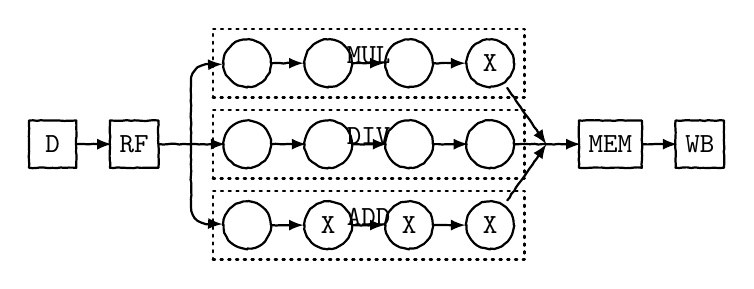
\begin{tikzpicture}[
    >=latex,thick,
    /pgf/every decoration/.style={/tikz/sharp corners},
    fuzzy/.style={decorate,
        decoration={random steps,segment length=0.5mm,amplitude=0.15pt}},
    minimum size=6mm,line join=round,line cap=round,
    terminal/.style={rectangle,draw,fill=white,fuzzy,rounded corners=3mm},
    nonterminal/.style={rectangle,draw,fill=white,fuzzy},
    node distance=4mm
  ]

    \ttfamily
    \begin{scope}[start chain,
            every node/.style={on chain},
            terminal/.append style={join=by {->,shorten >=-1pt,
                fuzzy,decoration={post length=4pt}}},
            nonterminal/.append style={join=by {->,shorten >=-1pt,
                fuzzy,decoration={post length=4pt}}},
            support/.style={coordinate,join=by fuzzy}
        ]
        \node [nonterminal]                        {D};
        \node [nonterminal]                        {RF};
        \node [support]   (before)    {};
        \node [terminal]  (stg1)      {};
        \node [terminal]  (stg2)      {};
        \node [terminal]  (stg3)      {};
        \node [terminal]  (stg4)      {};
        \node [support]   (after)     {};
        \node [nonterminal]                        {MEM};
        \node [nonterminal]                        {WB};
    \end{scope}
    \node (mul1)  [terminal,above=of stg1] {};
    \node (add1) [terminal,below=of stg1] {};
    \node (mul2)  [terminal,above=of stg2] {};
    \node (add2) [terminal,below=of stg2] {X};
    \node (mul3)  [terminal,above=of stg3] {};
    \node (add3) [terminal,below=of stg3] {X};
    \node (mul4)  [terminal,above=of stg4] {X};
    \node (add4) [terminal,below=of stg4] {X};
    
    \node[draw,dotted,fit=(mul1) (mul2) (mul3) (mul4)] {MUL};
    \node[draw,dotted,fit=(stg1) (stg2) (stg3) (stg4)] {DIV};
	\node[draw,dotted,fit=(add1) (add2) (add3) (add4)] {ADD};
	
    \begin{scope}[->,decoration={post length=4pt},rounded corners=2mm,
            every path/.style=fuzzy]
     \draw (before) -- +(0,1) -- (mul1);
     \draw (before) -- +(0,-1) -- (add1);
     \draw (mul1) -- (mul2);
     \draw (mul2) -- (mul3);
     \draw (mul3) -- (mul4);
     \draw (add1) -- (add2);
     \draw (add2) -- (add3);
     \draw (add3) -- (add4);
     \draw (mul4) --  (after);
     \draw (add4) -- (after);
     
    \end{scope}
\end{tikzpicture}

Proposal B:
\tikzset{
  nonterminal/.style={
    % The shape:
    rectangle,
    % The size:
    minimum size=6mm,
    % The border:
    very thick,
    draw=red!50!black!50,         % 50% red and 50% black,
                                  % and that mixed with 50% white
    % The filling:
    top color=white,              % a shading that is white at the top...
    bottom color=red!50!black!20, % and something else at the bottom
    % Font
    font=\itshape
  },
  terminal/.style={
    % The shape:
    rounded rectangle,
    minimum size=6mm,
    % The rest
    very thick,draw=black!50,
    top color=white,bottom color=black!20,
    font=\ttfamily},
  skip loop/.style={to path={-- ++(0,#1) -| (\tikztotarget)}}
}

{
  \tikzset{terminal/.append style={text height=1.5ex,text depth=.25ex}}
  \tikzset{nonterminal/.append style={text height=1.5ex,text depth=.25ex}}
}

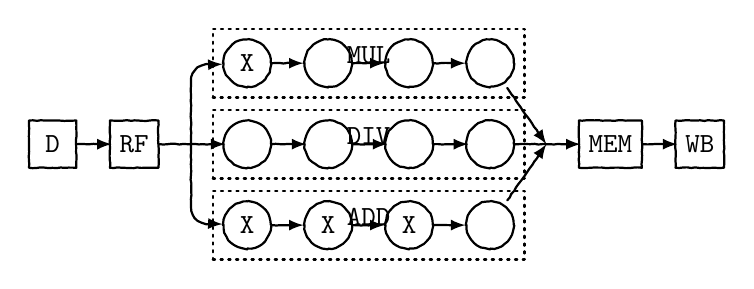
\begin{tikzpicture}[
    >=latex,thick,
    /pgf/every decoration/.style={/tikz/sharp corners},
    fuzzy/.style={decorate,
        decoration={random steps,segment length=0.5mm,amplitude=0.15pt}},
    minimum size=6mm,line join=round,line cap=round,
    terminal/.style={rectangle,draw,fill=white,fuzzy,rounded corners=3mm},
    nonterminal/.style={rectangle,draw,fill=white,fuzzy},
    node distance=4mm
  ]

    \ttfamily
    \begin{scope}[start chain,
            every node/.style={on chain},
            terminal/.append style={join=by {->,shorten >=-1pt,
                fuzzy,decoration={post length=4pt}}},
            nonterminal/.append style={join=by {->,shorten >=-1pt,
                fuzzy,decoration={post length=4pt}}},
            support/.style={coordinate,join=by fuzzy}
        ]
        \node [nonterminal]                        {D};
        \node [nonterminal]                        {RF};
        \node [support]   (before)    {};
        \node [terminal]  (stg1)      {};
        \node [terminal]  (stg2)      {};
        \node [terminal]  (stg3)      {};
        \node [terminal]  (stg4)      {};
        \node [support]   (after)     {};
        \node [nonterminal]                        {MEM};
        \node [nonterminal]                        {WB};
    \end{scope}
    \node (mul1)  [terminal,above=of stg1] {X};
    \node (add1) [terminal,below=of stg1] {X};
    \node (mul2)  [terminal,above=of stg2] {};
    \node (add2) [terminal,below=of stg2] {X};
    \node (mul3)  [terminal,above=of stg3] {};
    \node (add3) [terminal,below=of stg3] {X};
    \node (mul4)  [terminal,above=of stg4] {};
    \node (add4) [terminal,below=of stg4] {};
    
    \node[draw,dotted,fit=(mul1) (mul2) (mul3) (mul4)] {MUL};
    \node[draw,dotted,fit=(stg1) (stg2) (stg3) (stg4)] {DIV};
	\node[draw,dotted,fit=(add1) (add2) (add3) (add4)] {ADD};
	
    \begin{scope}[->,decoration={post length=4pt},rounded corners=2mm,
            every path/.style=fuzzy]
     \draw (before) -- +(0,1) -- (mul1);
     \draw (before) -- +(0,-1) -- (add1);
     \draw (mul1) -- (mul2);
     \draw (mul2) -- (mul3);
     \draw (mul3) -- (mul4);
     \draw (add1) -- (add2);
     \draw (add2) -- (add3);
     \draw (add3) -- (add4);
     \draw (mul4) --  (after);
     \draw (add4) -- (after);
     
    \end{scope}
\end{tikzpicture}

Where \texttt{X} designates a dummy stage.  The latency is thus 6 cycles before a result is available for data forwarding.
\end{solution}

\begin{problem}[3b]
Explain why both solutions ensure in-order updates to the registers.
\end{problem}

\begin{solution}
Both proposals constrain the three function units to complete in exactly the same number of cycles, which insures the results of the operations reach the \texttt{MEM} stage in precisely the same order in which they were issued to the FU, resulting in in-order register updates.
\end{solution}

\begin{problem}[3c]
Assuming that each proposal is implemented with forwarding logic in place, compare and contrast these two solutions.
\end{problem}

\begin{solution}
The benefits of either proposal would, in part, depend on the typical load and instruction order the pipeline will receive.  If either \texttt{MUL} or \texttt{ADD} are waiting on \texttt{DIV}, Proposal B seems more beneficial: during the dummy stages, these instructions would be stalled anyway, waiting for the result from \texttt{DIV}.  This way, \texttt{ADD} would need only one additional cycle, though \texttt{MUL} would need 3.

On the other hand, with Proposal A, a \texttt{DIV} waiting on either \texttt{MUL} or \texttt{ADD} would be able to have its result forward more quickly, decreasing the latency of that dependency.   
\end{solution}

\begin{problem}[3d]
Estimate the total number of comparators needed in either design to forward register operand values to waiting instructions.  \texttt{MUL}, \texttt{DIV}, other logical and arithmetic operations and \texttt{LOAD} all have at most 2 source registers each, while \texttt{STORE} can have up to 3 source registers.  Do not consider forwarding from a \texttt{LOAD} to a \texttt{STORE}.
\end{problem}

\begin{solution}
We will first need the four comparators originally discussed in the lecture on the forwarding unit. These will cover, for example, cases where \texttt{ADD} or \texttt{MUL} is \texttt{DIV} to finish execution and reach the \texttt{MEM} stage.  Comparators will also be needed for inter-unit forwarding.  For instances, an \texttt{ADD} or \texttt{MUL} may finish early and be able to stop a \texttt{DIV} from stalling and proceed with execution.  This adds an additional 6 (two per FU).  We will thus need approximate 10 comparators in our forwarding unit to properly dispatch values.
\end{solution}
\end{document}
